\documentclass{book}

\title{Design Document}
\author{Christian Stricker \and David Klopp \and Markus Vieth}
\date{\today}


\begin{document}
\frontmatter
\maketitle
\tableofcontents
\mainmatter
\part{Architectural Design}

\chapter{Introduction}
 Im Folgenden werden in diesem Dokument verschiedene Perspektiven des zu entwickelnden Systems betrachtet. Dazu wird das System in Teilsysteme zerlegt und deren Verhalten aufgezeigt.\\
\\
Das System, sowie alle Angaben zum System, beziehen sich dabei auf das "`Requirements Document for TODO"' vom 20. November 2015.
 
 %Siehe Kapitel 5 Sommerville
\chapter{External Layer} %Stakeholderanalyseartig (Umgebung des Systems) UML Activity Diagramm
Das System, als Web-Applikation, interagiert mit anderen Systemen in seiner Umgebung. TODO kommuniziert zur Übertragung von Daten mit mehreren Clients, welche Anfragen senden und Antworten empfangen, und mit weiteren Servern um Daten in den Datenbanken auszutauschen.\\
\begin{figure}[h]
	\vspace{-10pt}
\centering
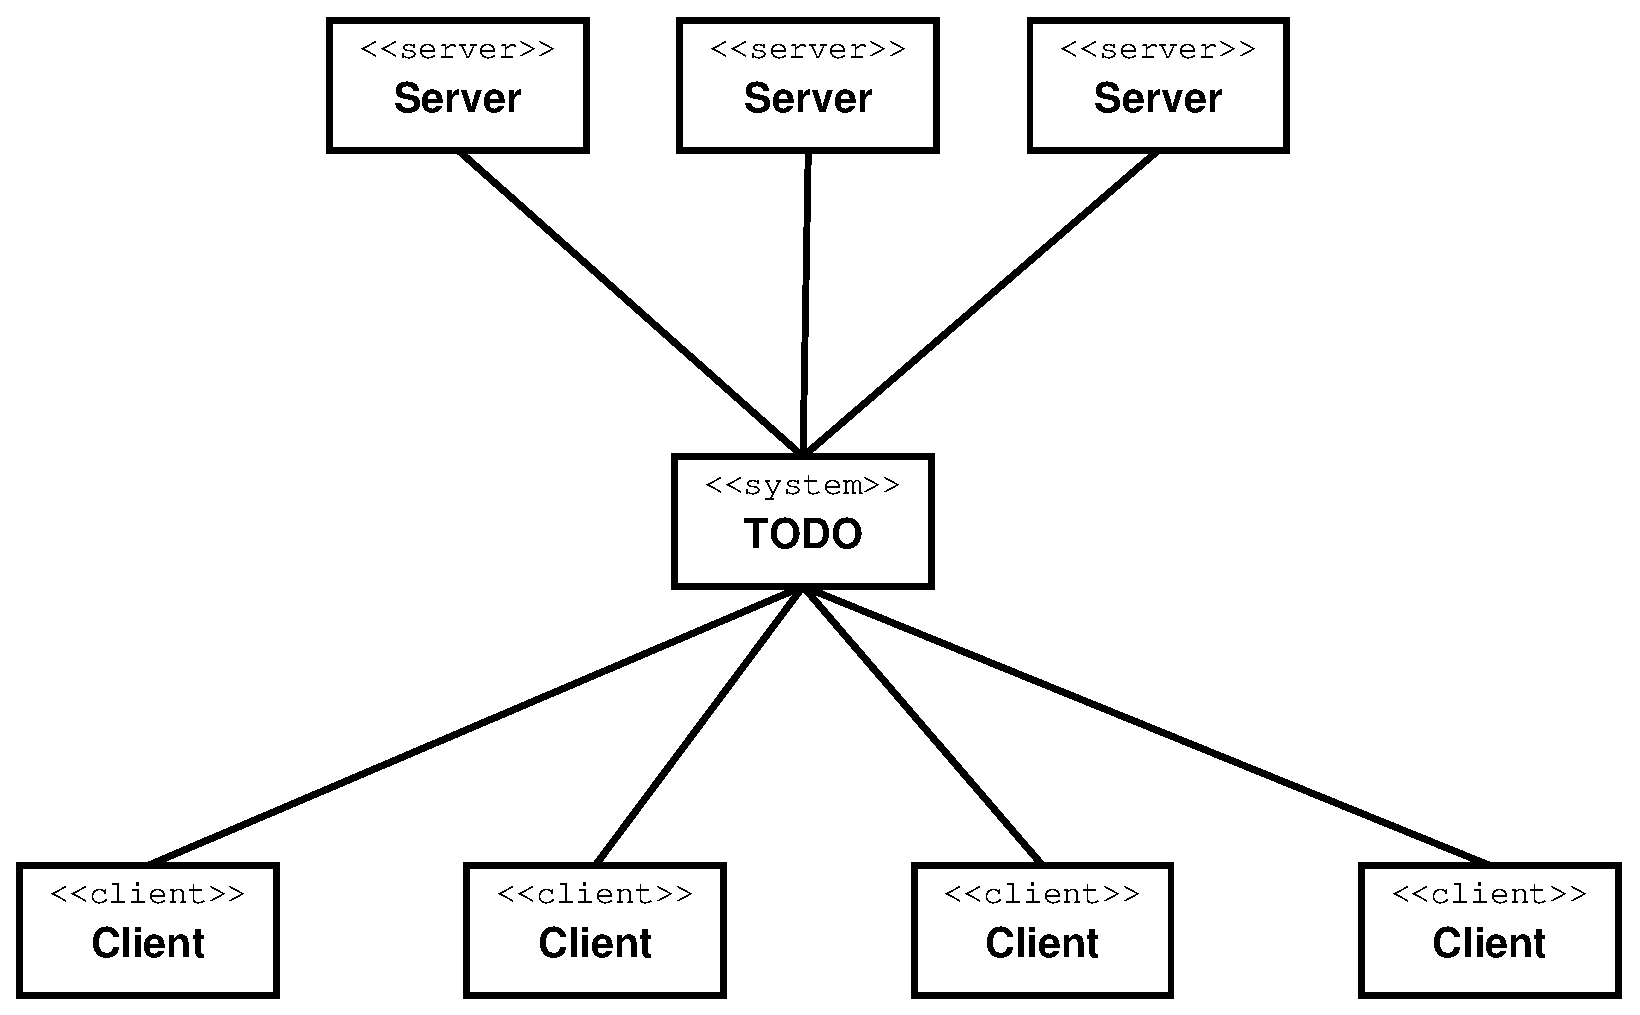
\includegraphics[width=0.9\linewidth]{Grafik/Diagramm/External}
\caption[Context Diagram]{Context Diagram des Systems im Bezug zu seiner Umgebung}
\label{fig:External}
\end{figure}\\
Die Kommunikation zwischen dem TODO und anderen Servern läuft dabei über das REST-Interface ab. Auch die Clients nutzen REST um Anfragen an das System zu stellen. Die Verbindung wird über HTTPS aufgebaut. Der Nutzer kann zur Kommunikation mit dem System jegliche Software nutzen, welche den Austausch von Daten über HTTPS unterstützt, insbesondere Browser wie Firefox oder Google Chrome. Ein Administrator hat die Möglichkeit über einen Client oder direkt an dem Rechner, auf dem das System läuft, zu arbeiten.
\chapter{Interaction Layer} %Ineraktion zwischen Umgebung und System, sowie zwischen einzelnen Modulen intern. Mit Use-case UML diagrammen und Sequence UML Diagrammen
%Hier würde, denke ich, das Pattern Zeug ganz gut rein passen. 
\chapter{Structural Layer} %Struktur der Daten UML Object-Diagramme, Generalisierungs Hierachy
\chapter{Behavioral Layer} %Verhalten des Systems und Reaktion auf Events UML State-Diagramme


\chapter{\ldots}
 
\end{document}

%%% Local Variables:
%%% mode: latex
%%% TeX-master: t
%%% End:
